\section{On the theory of fitting}


\subsection{Quantile-Density Based Metrics}
Following \cite{staudte2017dqf}, we construct the notion of Divergences based on the density-quantile function $dq(p) = f(F^{-1}(p)) \quad \forall p \in [0,1]$. The advantages of calculating divergence metrics on this transformed domain is that divergences become location-scale invariant and invariant to ``flat'' regions in the CDF.


\subsection{Divergence Density/Potential}
For some target density $g$, if its divergence $D_g(f)$ from any candidate density $f$ can be represented as the integral
\[\int_{x \in \mathcal X} L(f(x),g(x)) \d x\]
then define:
\[V(x,y) = L(y, g(x))\]
as the divergence density/potential associated with $g$ and induced by $L$. It gives a glimpse at the topography of penalization of $D(\cdot, \cdot)$ with respect to $g$. This is a useful metric if we want to compare how different tuning parameter $\alpha$'s affect the DPD.
\begin{figure}[h!]
	\centering
	
\includegraphics[width=0.7\linewidth]{fig/3-divpot.png}
	\caption{Divergence Potential associated with $\Sinu(1,1)$ and induced by the Hellinger distance}
	\label{fig:divpot}
\end{figure}
The process of fitting a candidate distribution over a given target then becomes merely an act of minimizing the line integral of potential function along the density line whilst ensuring that the area under the density line is 1.

We can conclude that the \sindist{} is indeed more flexible if for different target densities, which may even come from data, it can minimize the divergence better than conventional distributions. At the same time, excess efficiency implies lack of robustness in the presence of contamination. In such cases, we justify the utility of the \sindist{} by saying that it fits to data more flexibly than other distributions, and transparently displays the nature of the underlying divergence metric without interference from the rigidity of its shape.

\begin{table}
	\begin{tabular}{c|c|c}
		Divergence name  &  Potential $L_g(y)$  &  Gradient $\nabla_y L_g(y)$\\
		\hline
		Hellinger  &  $\frac{1}{2} (\sqrt y - \sqrt g)^2$  &  $\frac{1}{2 \sqrt y} (\sqrt y - \sqrt g)$\\
		DPD  &  $f^\alpha(f-g) - \frac{1}{\alpha}g(f^\alpha - g^\alpha)$  &  $(1+\alpha) y^{\alpha-1} (y-g)$\\
	\end{tabular}
\end{table}

Almost all divergences are functions of $y-g$, i.e. dependent on the deviation.

\subsubsection{DPD and contamination}
Higher $\alpha$ causes a lower rate of increase of penalization for deviating from true curve, thereby providing more feasibility of a fit that covers both density portions. Whereas a lower $\alpha$ allows rigid maximization over one of the 2 curves only, since passing through the middle high-penalization region in between incurs a lot of cost. See \autoref{fig:dpdpots}.

   \begin{figure}[h]
	\begin{subfigure}{0.49\linewidth}
		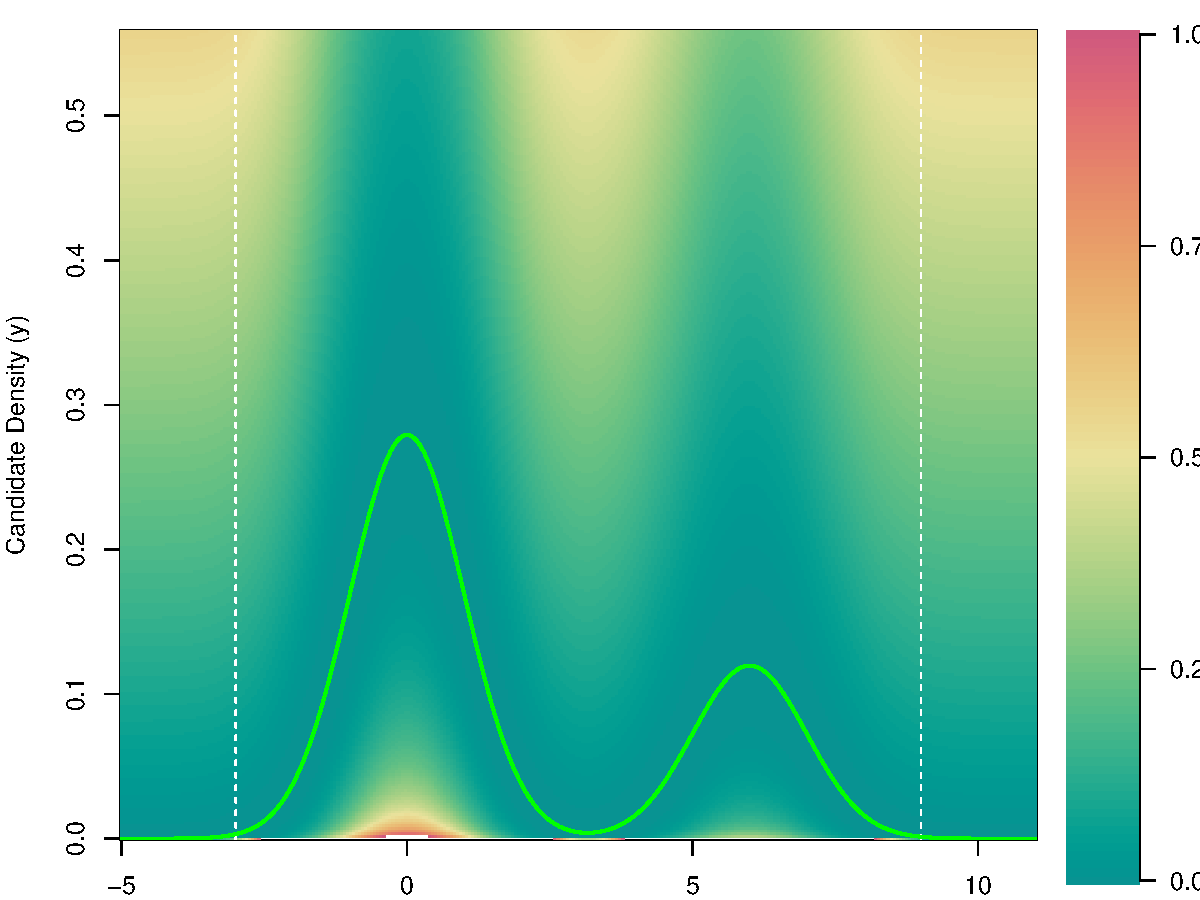
\includegraphics[width=\linewidth]{fig/divpot contamin 0.01}
		\caption{$\alpha=0.01$}
	\end{subfigure}
	\begin{subfigure}{0.49\linewidth}
		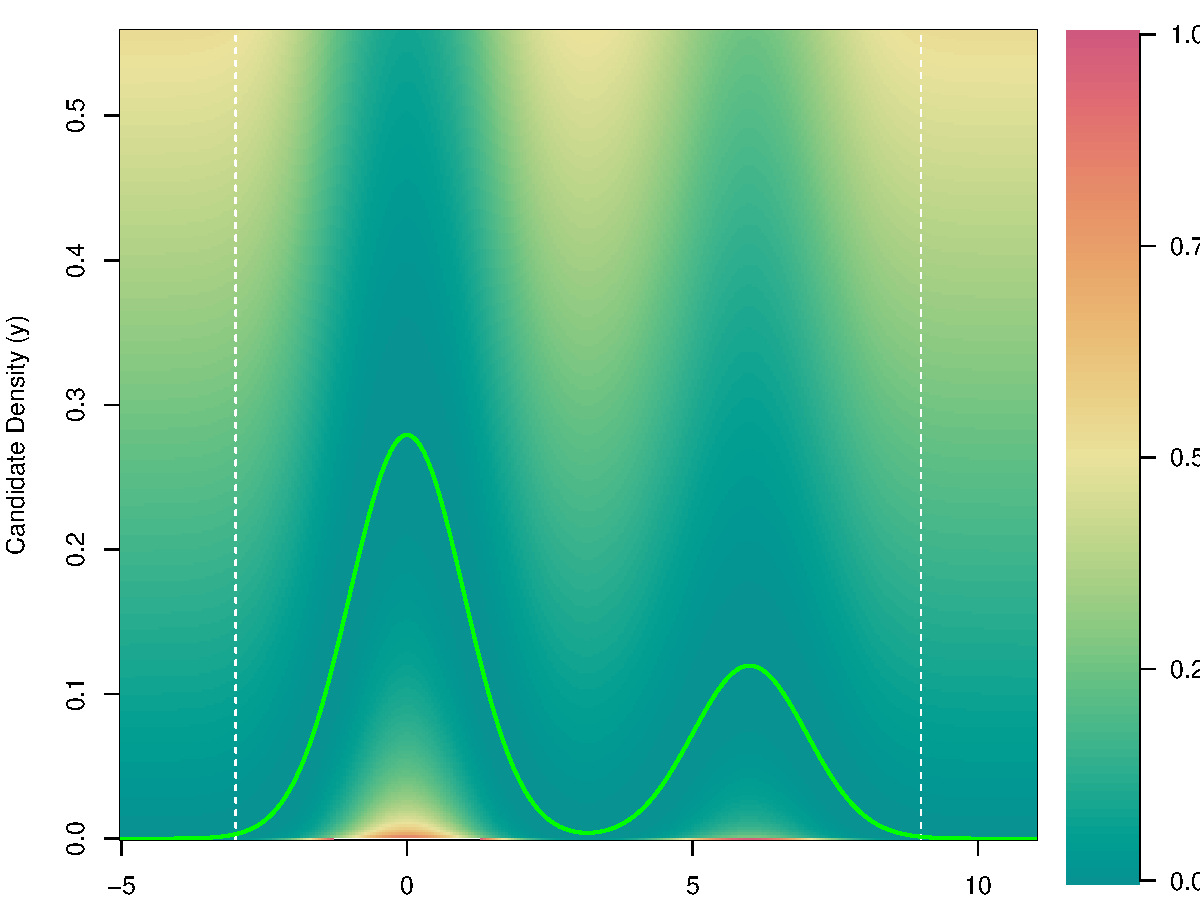
\includegraphics[width=\linewidth]{fig/divpot contamin 0.1}
		\caption{$\alpha=0.1$}
	\end{subfigure}
	\begin{subfigure}{0.49\linewidth}
		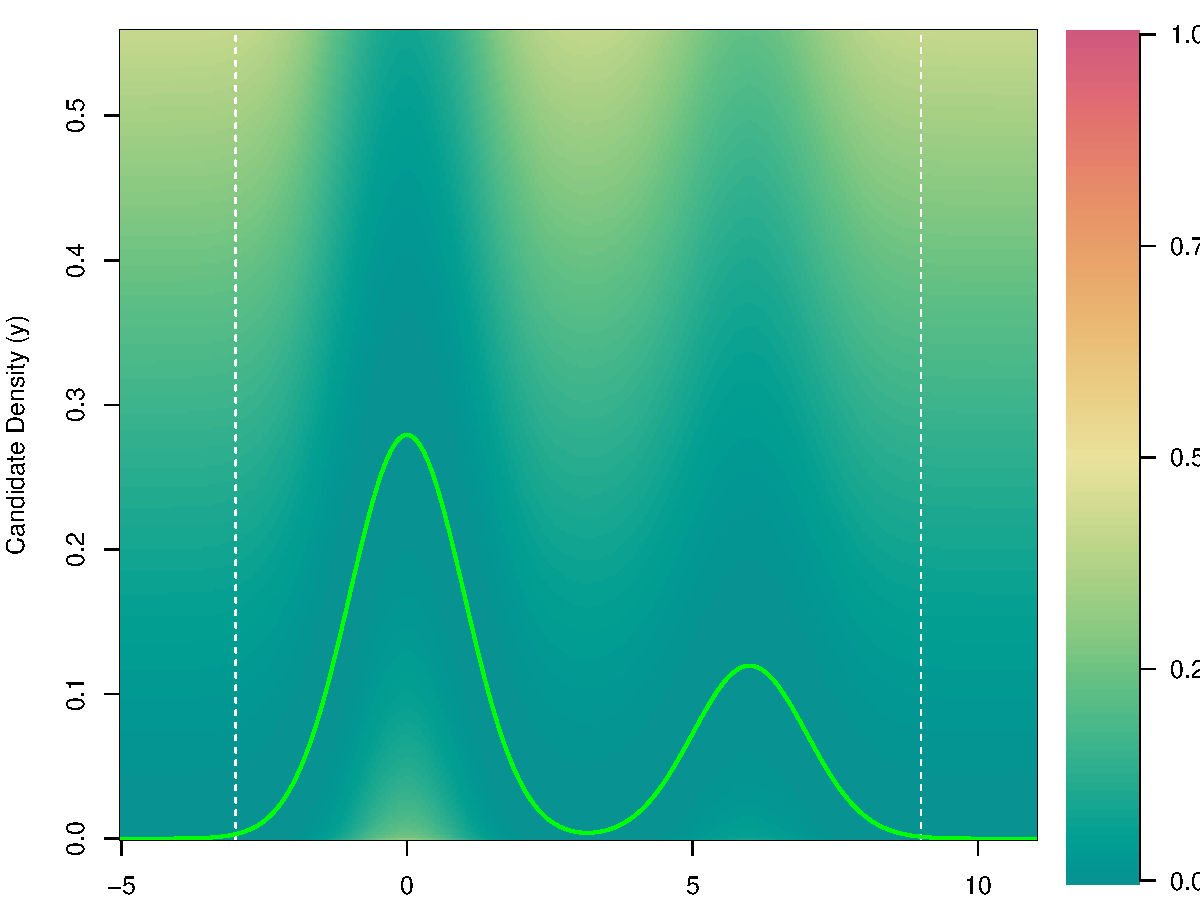
\includegraphics[width=\linewidth]{fig/divpot contamin 0.5}
		\caption{$\alpha = 0.5$}
	\end{subfigure}
	\begin{subfigure}{0.49\linewidth}
		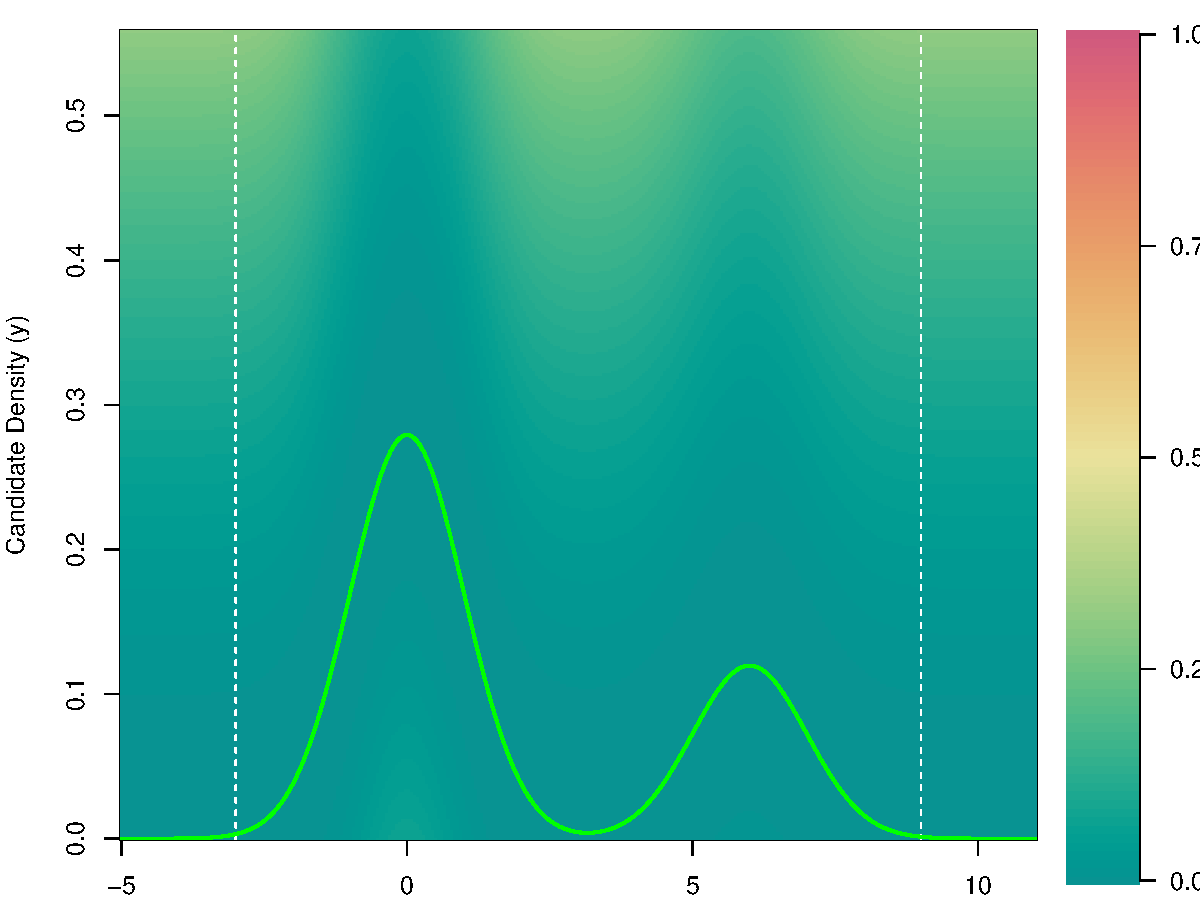
\includegraphics[width=\linewidth]{fig/divpot contamin 1}
		\caption{$\alpha = 1$}
	\end{subfigure}
	\caption{Shape plots of different \sindist s}\label{fig:dpdpots}
\end{figure}

In the presence of contamination, there is the additional complexity of the principal density being scaled down. So even if the distribution were to fit to the principal density portion, it would it to a dwarved version of it, thereby adjusting a best fit over its ``cloud" of minimality. Thereby the candidate distribution is now betrayed to fit over a ``non-density" principal component.

Finally observe that for contaminated densities, it is not the ``attraction'' of the second peak that deviates the candidate to fit contaminatedly, but it is the infeasibility in between that makes unimodal densities suboptimal fits, thereby seeking that the candidate choose either the principal or the contaminant density component.

\subsubsection{Calculus of variations}
We will work in the DQF domain so as to eliminate the question of location-scale dependence. We are looking at the problem:

\[ \inf_{s,k} \int_{y=\psi^*(x;s,k)} L_g(\psi^*(x)) \d x \]
\[\inf_{s,k} \int_{\mathcal{C}: y=\psi^*(x; s,k)} \frac{L(y, g(x))}{\sqrt{(1 + y')^2}} \, ds\]


Suggestion: A heuristic method to check feasibility of fitting
\begin{enumerate}
	\item For a contaminated density, choose the local maxima. Call the principal density's maximum $x_0$, and the subsequent ones $x_1, x_2, \dots$. We will assume a simple additional unimodal contamination, at $x_1$.
	\item Draw a straight line through the peaks. Find the ``deepest gorge" along this line and ascertain the potential at that point. Call it $L_{01}$. Call the length of the line $l_{01}$.
	\item Maybe put some sort of a threshold on the value of $L_{01}$ and $l_{01}$ based on whether the candidate density fits principally or contaminatedly.
	\item Problems: Not sure if this is a universal approach. Works for unimodal candidate densities, heuristically. Unsure if even then, $s,k$ will spoil the consistency. Or how the separation $l_{01}$ affects the threshold. Ideally, $\alpha$ should not affect the threshold: after all, our task is to ascertain the correct choice of $\alpha$ using the threshold and the graphical details alone of the potential map.
\end{enumerate}